% !TEX root = ../notes_missingsemester.tex
% Chapter 6: Data Lives Here — Databases & SQL
%%%%%%%%%%%%%%%%%%%%%%%%%%%%%%%%%%%%%%%%%%%%%%%%%%%%%%%%%%%%%%%%%%%%%%

% POST IMPROVEMENTS 2026:
% 1. Add a small TikZ schema diagram of the predictions table.
% 2. Provide a pre-baked v0.4 reference repo so catch-up takes a single clone.

\index{SQLite}\index{SQL}\index{SQLAlchemy}\index{database}\index{Alembic}\index{ORM}\index{PostgreSQL}
\chapter{Databases \& SQL}
\printchapterversion{06_databases_sql}
\newthought{In Comparison, Dumbledore's Pensieve is a joke.}

% ==============================================================================================
% BLOCK 1: INTRODUCTION
% ==============================================================================================

\section{The Why}\index{persistence}\index{relational database}


\marginnote{\newthought{SQLAlchemy.}\index{SQLAlchemy}\index{ORM}\index{SQL}
The Object-Relational Mapper, abbreviated ORM, that bridges Python
objects and relational tables. You write Python classes; SQLAlchemy
generates the Structured Query Language, abbreviated SQL, behind them,
so the handler talks to the database without composing query strings
by hand.\\
\url{https://www.sqlalchemy.org/}}


We have a service that classifies, but it does not remember anything.
The moment the response leaves the server, the prediction is gone.
This makes it hard to track the model's performance over time, compare versions, or
build any type of features and functionality that revolve around
past predictions.

\newthought{We need to wire the API onto a database.}\index{PixelWise}
This block is the first that adds persistent state.
Every later block depends on the database schema you design today.

\begin{figure}
\centering
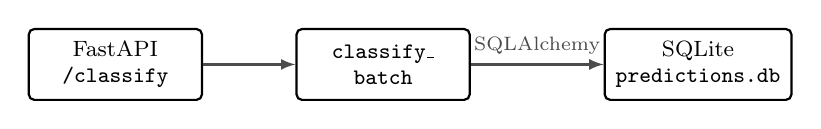
\begin{tikzpicture}[
    every node/.style={font=\footnotesize, align=center},
    box/.style={rectangle, draw=black, thick, rounded corners=2pt, minimum width=2.2cm, minimum height=0.9cm, inner sep=4pt},
    arr/.style={-latex, thick, black!70}
]
\node[box] (api) at (0, 0)    {FastAPI\\\texttt{/classify}};
\node[box] (cb)  at (3.4, 0)  {\texttt{classify\_}\\\texttt{batch}};
\node[box] (pg)  at (7.4, 0)  {SQLite\\\texttt{predictions.db}};
\draw[arr] (api.east) -- (cb.west);
\draw[arr] (cb.east)  -- node[above]{\scriptsize SQLAlchemy} (pg.west);
\end{tikzpicture}
\caption{The persistence flow. \texttt{POST /classify} computes a prediction with \texttt{classify\_batch}, the handler maps the result through the \texttt{Prediction} SQLAlchemy model, and a row lands in the \texttt{predictions} table inside the \texttt{predictions.db} SQLite file before the response goes out.}
\label{fig:persistence_flow}
\end{figure}





\newthought{Why persist at all?}
A response that vanishes the moment it is sent is a response that cannot be
counted, compared, or queried.
A database makes the prediction permanent: Every drawing becomes a row, the
class label becomes a column, the confidence becomes another, and the model
version becomes a third.

\newthought{Beyond this course,}
the same table is where production teams build retraining datasets, let
users correct wrong predictions for labelled data, and detect distribution
drift.
We do not do any of those here, but it is trivial to see how every one of them starts with having
the database.



\newpage
\subsection{Hands On Experience}

\newthought{Consider this scenario:} A teammate asks how confident the
model has been on average across the last hundred predictions.
You realise nobody can answer that question.
The API returned the confidence to every caller, but nothing recorded it.
The only way back to those numbers is to ask the users to draw their digits
again, which is not an option. In an increasingly data-driven world, data defines your product, 
your moat, and your competitive advantage. Not having the data is like throwing away your most valuable asset, and 
until someone comes up with a solution for time-travel, it's a non-recoverable loss.

\newthought{The schema is a contract,} the same way the API contract is a
contract.
Get it right and every later question, distribution per digit, average
confidence per model version, error rate over time, becomes a query.
Get it wrong and you find out later, with a hundred thousand rows already
written, that the column you need does not exist.
We keep the schema small and deliberate from the start, so the columns
worth having are there before any rows are.

\marginnote{\newthought{Designing schemas} is its own discipline.
We start with a small, deliberate schema, four columns, that covers
everything later blocks need to read back.
The point is to feel the cycle of design and deploy on a real database,
not to ship a kitchen-sink table on day one.}

\newthought{This sixth block} introduces persistence for PixelWise.
By the end you will have
\begin{itemize}
    \item written your first SQL queries against a SQLite database,
    \item modelled the \texttt{predictions} table as a SQLAlchemy class,
    \item wired \texttt{POST /classify} so every prediction becomes a row,
    \item replaced the \texttt{GET /results} stub with a real query,
    \item pointed the application at the database through \texttt{.env},
    \item and, optionally, run your first schema migration with Alembic.
\end{itemize}



% ==============================================================================================
\newpage
\section{Optional Exercise: Catch Up to \texttt{v0.4}}\index{exercises}\index{Git!tag}\index{recovery}

\marginnote{\newthought{Tag map.}\index{Git!tag}
\texttt{v0.4} marks the end of Block~5, \texttt{v0.5} will mark the end
of this block.
Browse the full set at
\url{https://github.com/schutera/pixelwise/tags}.}

\newthought{Catching up via tag.}\index{Git!tag}\index{recovery}
This catch-up extends the one in Block~5. If you have not done that one,
do it first: It lands you at \texttt{v0.3}, the end-of-Block~4 state.
The exercise here picks up from there and rewinds to \texttt{v0.4}, the
end-of-Block~5 state, with the FastAPI service exposing
\texttt{POST /classify} and \texttt{GET /health}, API key authentication,
basic rate limiting, and a \texttt{systemd}-supervised \texttt{uvicorn}
running on \texttt{prod}.

\newthought{Both VMs this time.} Block~5 ended with the service actually
running on \texttt{prod}, so unlike the previous catch-up, this one
brings both machines up to \texttt{v0.4}. The Git-tracked changes since
\texttt{v0.3} include \texttt{app/main.py},
\texttt{deploy/pixelwise.service}, an extended \texttt{setup-server.sh}
that installs the systemd unit on \texttt{prod}, an updated
\texttt{requirements.txt} adding \texttt{fastapi}, \texttt{uvicorn},
\texttt{slowapi}, and \texttt{pydantic}, and a refreshed
\texttt{.env.example} with \texttt{SECRET\_API\_KEY}. The local
\texttt{.env} on \texttt{prod} needs the new key written by hand;
\texttt{setup-server.sh} then pulls the model, copies the unit,
enables, and restarts the service in one shot.

\newthought{Run the catch-up on \texttt{dev}.}
Rewind the repository to \texttt{v0.4}, refresh \texttt{.env} from the
updated example and edit it to set \texttt{SECRET\_API\_KEY}, reinstall
pinned dependencies if your virtual environment was wiped, then run
\texttt{setup-server.sh} to pull the model artefact. The exact commands
are in the margin.

\marginnote{\newthought{Sequence on \texttt{dev}.}\\[0.4em]
\texttt{cd \textasciitilde/pixelwise}\\
\texttt{git fetch origin -{}-tags}\\
\texttt{git reset -{}-hard v0.4}\\
\texttt{cp .env.example .env}\\
\texttt{nano .env}\\
\texttt{source .venv/bin/activate}\\
\texttt{pip install -r requirements.txt}\\
\texttt{bash setup-server.sh}\\[0.3em]
Edit \texttt{.env} to set \texttt{SECRET\_API\_KEY} to any string of
your choosing; \texttt{openssl rand -hex 32} prints a clean random
value if you want one.
If you already have a \texttt{.env} from earlier work, skip the
\texttt{cp} and just edit the file in place.
If \texttt{.venv/} is missing, run
\texttt{python3 -m venv .venv} before the \texttt{source} step.}

\newthought{Run the catch-up on \texttt{prod}.}
Same sequence on prod, where \texttt{setup-server.sh} also copies the
systemd unit into place and restarts the service. After the script
finishes, verify the API is reachable from \texttt{dev}.

\marginnote{\newthought{Sequence on \texttt{prod}.}\\[0.4em]
\texttt{ssh produser@192.168.56.11}\\
\texttt{cd /opt/pixelwise}\\
\texttt{git fetch origin -{}-tags}\\
\texttt{git reset -{}-hard v0.4}\\
\texttt{cp .env.example .env}\\
\texttt{nano .env}\\
\texttt{source .venv/bin/activate}\\
\texttt{pip install -r requirements.txt}\\
\texttt{bash setup-server.sh}\\[0.3em]
Use the same \texttt{SECRET\_API\_KEY} value as on \texttt{dev}.
If you already have a \texttt{.env} on \texttt{prod}, skip the
\texttt{cp} and edit the file in place.
Then from \texttt{dev}:
\texttt{curl http://192.168.56.11:8000/health}
should return \texttt{\{"status":"ok"\dots\}}.}


\newthought{You are now} at the state where Block~5 ended, with both
machines aligned, ready to start Block~6.



% ==============================================================================================
% BLOCK 2: CONCEPTS AND PRACTICE
% ==============================================================================================

\newpage
\section{Relational Databases and SQL}\index{relational database}\index{SQL}

\newthought{A relational database stores data in tables.}
Each table has a fixed schema: a list of named columns, each with a type.
Each row is a single record.
The schema is the contract that every row obeys; the database refuses
inserts that violate it.

\marginnote{\newthought{Vocabulary to keep straight.}\index{primary key}
A \emph{table} is a named set of rows; a \emph{row} is one record;
a \emph{column} is a named field with a type;
a \emph{primary key} is the column (or set of columns) that uniquely
identifies each row.
Most tables use an auto-incrementing integer or a UUID as their key.}

\newthought{SQL\index{SQL} is the language} you use to talk to a relational database.
Four operations cover almost everything:

\begin{verbatim}
-- Insert a row
INSERT INTO predictions (prediction, confidence,
                         model_version)
VALUES ('7', 0.94, 'v1');

-- Read rows
SELECT prediction, confidence FROM predictions
    WHERE model_version = 'v1'
    ORDER BY created_at DESC
    LIMIT 10;

-- Update a row
UPDATE predictions SET confidence = 0.95
    WHERE id = 42;

-- Delete a row
DELETE FROM predictions WHERE id = 42;
\end{verbatim}

\marginnote{\newthought{What you will meet later.}\index{SQL!JOIN}\index{SQL!GROUP BY}
\texttt{JOIN} combines rows from multiple tables;
\texttt{GROUP BY}, \texttt{COUNT}, and \texttt{AVG} aggregate;
\texttt{ORDER BY} and \texttt{LIMIT} shape the output;
\texttt{CREATE INDEX} speeds up queries that scan large tables.
The full treatment belongs in a dedicated database course; the four
operations above are enough to get PixelWise running.}

\newthought{The four operations are what every web application does to
its database all day long}: write a row when something happens, read rows
back when somebody asks, update a row when state changes, delete one when
it should be gone.
Every higher-level pattern, an ORM call, a migration, an analytics query,
reduces to a sequence of these.

\subsection{SQLite for this Course}\index{SQLite}\index{PostgreSQL}

\newthought{SQLite\index{SQLite} is a database in a single file.}
There is no server to install, no users, no passwords, no network
configuration.
The application opens the file, writes rows, closes the file.
For a course where one student runs one service on one VM, this is exactly
the right shape.

\marginnote{\newthought{What you give up.}
SQLite has no user authentication and limited concurrency: a single writer
blocks all readers.
For a multi-user production web service hit by hundreds of clients per
second, the file-lock model becomes the bottleneck, and a separate
database process becomes the right call.
For PixelWise with one user clicking through Swagger, the file is more than
enough.}

\newthought{PostgreSQL\index{PostgreSQL} is the production next step.}
It runs as a separate process, accepts network connections, has real users
with real permissions, and supports concurrent reads and writes without
serialising the whole file.
The shift from SQLite to PostgreSQL is mostly one line of
\texttt{DATABASE\_URL} plus the operational work of installing the server,
creating a role, and managing the password.
We stop one step short of that here; everything else in the chapter, the
SQLAlchemy model, the migrations, the queries, looks the same against
either backend.

\marginnote{SQLite: \url{https://www.sqlite.org/}\\
SQLite CLI docs: \url{https://www.sqlite.org/cli.html}\\
PostgreSQL: \url{https://www.postgresql.org/}}

\newthought{Setting up the database} is a one-liner: pick a file path,
and SQLAlchemy creates the file on first connect.
The application user is the OS user that owns the file; the privilege
model collapses to file-system permissions.
\texttt{sqlite3}\index{sqlite3} is the operator's interface, the same
shape of tool as \texttt{psql} for PostgreSQL or \texttt{systemctl} from
Block~5: a small REPL you drop into when you want to look at the data
behind the application.

\marginnote{\newthought{Where the file lives.}\index{file permissions}
On \texttt{prod} the database file sits inside
\texttt{/opt/pixelwise/}, owned by \texttt{produser}.
The same OS-level least-privilege story from Block~1 applies: the
application user owns the data file, no one else needs to read it, and a
backup is one \texttt{cp} of a single file.}



% ==============================================================================================
\newpage
\section{Exercise: SQLite on the Server}\index{exercises}\index{SQLite}

\marginnote{\newthought{Exercises} are where the theory becomes muscle
memory. SQLite needs almost no setup, so this first exercise is a
five-minute warm-up: pick a file path, make sure the directory exists,
verify with the \texttt{sqlite3} CLI. The substance comes in the next
two exercises where SQLAlchemy and the API land on top.}

\newthought{Install the \texttt{sqlite3} CLI on \texttt{prod}.}
The SQLite database engine itself ships as a Python C extension and
needs no separate install. The \texttt{sqlite3} command-line tool is a
small REPL useful for poking at the file by hand:

\begin{verbatim}
ssh produser@192.168.56.11
sudo apt update
sudo apt install -y sqlite3
sqlite3 --version
\end{verbatim}

\newthought{Pick a path for the database file.}\index{DATABASE\_URL}
The application user owns it, so it lives inside the application
directory. On \texttt{prod} that is \texttt{/opt/pixelwise/}; the file
will be created on first connect:

\begin{verbatim}
# on prod
ls -la /opt/pixelwise/
# /opt/pixelwise/pixelwise.db will appear here
# the first time the API or init_db.py runs
\end{verbatim}

\marginnote{\newthought{The connection string}\index{DATABASE\_URL} is a
single URL: \\
\texttt{sqlite:////absolute/path/to/file.db}.
Note the four slashes after the colon: three for the URL scheme, one
for the absolute path. A relative path uses three slashes
(\texttt{sqlite:///./pixelwise.db}). The application reads this from
\texttt{.env}, so the same code works on \texttt{dev} and \texttt{prod}
with different paths.}

\newthought{Add \texttt{DATABASE\_URL}} to both VMs' \texttt{.env} and
to the committed \texttt{.env.example}. The values differ per host, the
key does not:

\begin{verbatim}
# /opt/pixelwise/.env on prod
DATABASE_URL=sqlite:////opt/pixelwise/pixelwise.db

# ~/pixelwise/.env on dev
DATABASE_URL=sqlite:///./pixelwise.db

# .env.example, committed on dev
DATABASE_URL=sqlite:///./pixelwise.db
\end{verbatim}

\newthought{Verify the CLI works} against an empty database. The file
does not exist yet, so \texttt{sqlite3} creates it on the spot and
drops you into a prompt; \texttt{.tables} lists the empty schema and
\texttt{.quit} exits:

\begin{verbatim}
sqlite3 /opt/pixelwise/pixelwise.db
sqlite> .tables
sqlite> .quit
\end{verbatim}

The file now exists on disk with zero tables; the next exercise has
SQLAlchemy create the \texttt{predictions} table inside it.



% ==============================================================================================
\newpage
\section{SQLAlchemy: Tables as Python Classes}\index{SQLAlchemy}\index{ORM}

\newthought{SQLAlchemy is a Python library} that maps database tables to
Python classes.
You define a \texttt{Prediction} class with fields like \texttt{prediction},
\texttt{model\_version}, and \texttt{created\_at};
SQLAlchemy generates the SQL to create the table, insert rows, and query
data.
This is called an \emph{ORM}\index{ORM}, an object-relational mapper, and
is standard in Python web development.

\marginnote{SQLAlchemy: \url{https://www.sqlalchemy.org/}\\
SQLAlchemy Tutorial: \\
\url{https://docs.sqlalchemy.org/en/20/tutorial/}}

\newthought{The model class} declares the columns and their types in plain
Python.
A \texttt{Prediction} class inherits from a SQLAlchemy declarative base,
sets \texttt{\_\_tablename\_\_} to \texttt{predictions}, and lists each
column as a class attribute: An auto-incrementing integer primary key, a
non-null string for the predicted class, a non-null string for the model
version, and a timestamp that defaults to the current UTC time.
The exercise below has the full \texttt{app/models.py} the API will import.

\marginnote{\newthought{Why an ORM?}\index{SQL injection}
Two reasons.
The first is ergonomic: writing Python is faster than writing string SQL,
and the editor knows the field names.
The second is safety: SQLAlchemy uses parameterised queries by default,
which means user input never ends up concatenated into a SQL statement.
SQL injection becomes a footgun the framework refuses to hand you.}

\newthought{An engine and a session} are the runtime objects that connect
the model to the database.
\texttt{create\_engine} reads the \texttt{DATABASE\_URL} from the
environment and opens a pool of connections;
\texttt{sessionmaker} returns a \texttt{SessionLocal} factory the handlers
will call once per request;
\texttt{Base.metadata.create\_all(engine)} creates the table on first run.
The exercise wires these three lines into a small initialisation script
the team runs on \texttt{prod} before the first deploy.

\marginnote{\newthought{The connection string}\index{DATABASE\_URL} is a
single URL the engine parses: \\
\texttt{sqlite:////opt/pixelwise/pixelwise.db} on \texttt{prod}, the
matching relative form on \texttt{dev}.
It encodes everything the driver needs to reach the database, and it
lives in \texttt{.env} so the same code works against different files
on each host without code changes.}

\newthought{Inserting a row} from inside the API handler is now a few lines:
Open a session from \texttt{SessionLocal}, construct a \texttt{Prediction}
with the fields from the classifier result, add it to the session, and
commit.
The handler still calls \texttt{classify\_batch} from Block~4 and returns
\texttt{ClassifyResponse} from Block~5; the only addition is one round-trip
to the database before the response leaves the server.
The exercise below wires it up inside \texttt{POST /classify}.



% ==============================================================================================
\newpage
\section{Exercise: The \texttt{Prediction} Model}\index{exercises}

\newthought{Turn the theory above into code.}
On \texttt{dev}, install SQLAlchemy into the virtual environment from
the repository root. SQLite ships with the Python standard library, so
no separate driver is needed:

\begin{verbatim}
cd ~/pixelwise
source .venv/bin/activate
pip install sqlalchemy
pip freeze > requirements.txt
\end{verbatim}

\newthought{Write \texttt{app/models.py}} with the schema we will want to
read back later: the class label, the confidence, and the model version,
all stamped with a timestamp. From the repository
root on \texttt{dev}:

\begin{verbatim}
cd ~/pixelwise
nano app/models.py
\end{verbatim}

Paste the following, save with \texttt{Ctrl+O}, exit with \texttt{Ctrl+X}:

\begin{verbatim}
from sqlalchemy import (Column, Integer, String,
                        Float, DateTime)
from sqlalchemy.orm import declarative_base
from datetime import datetime

Base = declarative_base()

class Prediction(Base):
    __tablename__ = "predictions"
    id = Column(Integer, primary_key=True)
    prediction = Column(String, nullable=False)
    confidence = Column(Float, nullable=False)
    model_version = Column(String, nullable=False)
    created_at = Column(DateTime,
                        default=datetime.utcnow)
\end{verbatim}

\marginnote{\newthought{Why these four columns.}\index{schema}
The class label and confidence are what the model returns; the model
version lets you compare \texttt{v1} against future retrains; the
timestamp orders rows by recency.
Any later monitoring or analytics reads all four directly from this
table, so a complete schema today saves a migration later.}

\newthought{Create the table once} from a small initialisation script
saved as \texttt{init\_db.py} at the repository root on \texttt{dev}.
The script reads \texttt{DATABASE\_URL} you set in the previous
exercise and calls \texttt{Base.metadata.create\_all} to materialise
every model class into a table:

\begin{verbatim}
cd ~/pixelwise
nano init_db.py
\end{verbatim}

Paste the following:

\begin{verbatim}
from sqlalchemy import create_engine
from app.models import Base
import os
from dotenv import load_dotenv

load_dotenv()
engine = create_engine(os.getenv("DATABASE_URL"))
Base.metadata.create_all(engine)
\end{verbatim}

Commit and push from \texttt{dev}, then run the script on \texttt{prod}
where the database lives:

\begin{verbatim}
# on prod, after git pull
cd /opt/pixelwise
source .venv/bin/activate
python init_db.py
\end{verbatim}

Confirm with \texttt{sqlite3 /opt/pixelwise/pixelwise.db} that the
\texttt{.tables} command now lists \texttt{predictions}:

\begin{verbatim}
sqlite3 /opt/pixelwise/pixelwise.db
sqlite> .tables
predictions
sqlite> .schema predictions
sqlite> .quit
\end{verbatim}



% ==============================================================================================
\newpage
\section{Exercise: Wiring the API to the Database}\index{exercises}

\newthought{Update \texttt{app/main.py}} so \texttt{POST /classify} writes
a row before returning the response. Reopen the file from the repository
root on \texttt{dev}:

\begin{verbatim}
cd ~/pixelwise
nano app/main.py
\end{verbatim}

The handler from Block~5 stays the same shape; one new dependency creates
a database session per request:

\begin{verbatim}
from app.models import Prediction, SessionLocal

@app.post("/classify",
          response_model=ClassifyResponse,
          dependencies=[Depends(verify_api_key)])
def classify(req: ClassifyRequest):
    arr = np.array(req.pixels,
                   dtype=np.uint8)[np.newaxis]
    result = classify_batch(arr)[0]

    db = SessionLocal()
    db.add(Prediction(
        prediction=result["prediction"],
        confidence=result["confidence"],
        model_version="v1"))
    db.commit()
    db.close()

    return result
\end{verbatim}

\marginnote{\newthought{One session per request.}\index{SQLAlchemy!session}
A session is the unit of database work.
Open it at the start of the handler, close it at the end.
The framework patterns FastAPI documents (\texttt{Depends} for sessions)
do this more elegantly; the manual version above is the simplest one that
shows what is happening.}

\newthought{Replace the \texttt{GET /results} stub} in the same
\texttt{app/main.py} with a real query:

\begin{verbatim}
@app.get("/results")
def results():
    db = SessionLocal()
    rows = (db.query(Prediction)
              .order_by(Prediction.created_at.desc())
              .limit(20).all())
    db.close()
    return {"results": [
        {"id": r.id,
         "prediction": r.prediction,
         "confidence": r.confidence,
         "model_version": r.model_version,
         "created_at": r.created_at.isoformat()}
        for r in rows]}
\end{verbatim}

\newthought{Restart the service and feed it data.}
There is no browser canvas yet, so trigger predictions the same way as in
Block~5: through Swagger at
\texttt{http://192.168.56.11:8000/docs}, with the API key in the
\texttt{x\_api\_key} field and a zero-filled 28-by-28 body in the request
body. After a handful of calls,
\texttt{curl http://192.168.56.11:8000/results} from \texttt{dev} returns
the rows you just wrote, each with its class, confidence, model version,
and timestamp.
The stub from Block~5 is now complete; the system stores what it predicts.

\newthought{Commit and tag as \texttt{v0.5}.}
The repository now matches the end-of-Block~6 state that later catch-up
exercises rewind to. From the repository root on \texttt{dev}:

\begin{verbatim}
cd ~/pixelwise
git add app/main.py app/models.py init_db.py \
    requirements.txt .env.example
git commit -m "Add SQLite persistence via SQLAlchemy"
git push
\end{verbatim}

\marginnote{\newthought{Why stop here.}\index{schema}
The schema covers everything we will want to read back later, and the
service stores what it predicts.
Anything that comes after can sit on top of this state without needing
further database work.
The optional Alembic section that follows shows how schemas evolve once
real rows already exist; nothing in the core path depends on it.}



% ==============================================================================================
\newpage
\section{Optional: Schema Migrations with Alembic}\index{Alembic}\index{migration}

\marginnote{\newthought{Optional.}
Nothing in the core path depends on this section. The schema you shipped
at \texttt{v0.5} already carries every column later parts of the course
will want to read back. Run this section if you want to feel the
migration cycle on a live database; skip it otherwise.}

\newthought{Schemas always change.}
You design the table, deploy it, store 500 predictions.
Then you realise you forgot a column, or want to capture a new fact about
each row, like a human annotator's notes on whether the prediction was
correct.
You cannot drop the table and recreate it; those 500 rows are real data.
You need a tool that alters the live schema without losing them.

\marginnote{Alembic: \url{https://alembic.sqlalchemy.org/}\\
\newthought{The metaphor.}\index{migration}
A migration is a recipe that describes a change to the schema and how to
roll it back.
The migration tool keeps an internal log of which migrations have run,
applies new ones in order, and refuses to run the same one twice.
The result is that the schema in the database always matches the
migrations folder in Git.}

\newthought{Alembic} is the migration tool for SQLAlchemy.
It generates migration scripts from changes you made to the model,
applies them in order, and tracks which migrations have run on which
database.
The cycle is three commands: \texttt{alembic init} once per repository
to lay down the migrations folder, \texttt{alembic revision -{}-autogenerate}
after every model edit to draft the migration, and \texttt{alembic upgrade
head} to apply it.
The exercise below runs the full cycle to add a \texttt{notes} column for
human annotations on individual predictions.

\marginnote{\newthought{The autogenerate is a draft, not a final answer.}
Alembic compares the model in code against the schema in the database and
guesses what changed.
For straightforward additions it gets it right; for renames or splits it
needs a human to read the generated script and adjust it.
Always read the migration before you run it.}

\newthought{In a real system} with millions of rows and live traffic, you
cannot just drop and recreate.
Migrations are how schemas evolve safely, in production, with the
application running.
This topic is covered in much more depth in dedicated database and backend
courses; here we run one migration end to end so the cycle of edit-model,
generate-migration, apply-migration is concrete.

\marginnote{\newthought{Sidenote: Redis.}\index{Redis}
Redis is an in-memory key-value store with sub-millisecond reads.
It is the right tool for caching, session storage, and rate-limit counters.
For PixelWise, every drawing is unique pixel data, so the cache hit rate
would be effectively zero; we mention it so you recognise it later.\\
Redis: \url{https://redis.io/}}



% ==============================================================================================
\newpage
\section{Optional Exercise: First Migration with Alembic}\index{exercises}

\newthought{Initialise Alembic in the repo.}
With the migration cycle from the theory above in mind, configure the
tool to use the same engine as the application. \texttt{alembic init}
writes its scaffold into the current directory, so run everything from
the repository root on \texttt{dev}:

\begin{verbatim}
cd ~/pixelwise
source .venv/bin/activate
pip install alembic
pip freeze > requirements.txt
alembic init alembic
\end{verbatim}

Edit \texttt{alembic.ini} so \texttt{sqlalchemy.url} reads from
\texttt{.env}, and edit \texttt{alembic/env.py} to import \texttt{Base}
from \texttt{app.models} so autogenerate sees your tables.

\marginnote{\newthought{Read the generated config.}\index{alembic.ini}
\texttt{alembic init alembic} writes a folder of starter files.
Skim them once before you change anything; the structure is small and the
mental model becomes obvious by reading the templates.}

\newthought{Add a new column} to the model. Reopen
\texttt{app/models.py} from \texttt{\textasciitilde{}/pixelwise} on
\texttt{dev} and add a nullable \texttt{notes} field for free-form human
annotation of individual predictions:

\begin{verbatim}
cd ~/pixelwise
nano app/models.py
\end{verbatim}

\begin{verbatim}
class Prediction(Base):
    __tablename__ = "predictions"
    id = Column(Integer, primary_key=True)
    prediction = Column(String, nullable=False)
    confidence = Column(Float, nullable=False)
    model_version = Column(String, nullable=False)
    notes = Column(String)                # NEW
    created_at = Column(DateTime,
                        default=datetime.utcnow)
\end{verbatim}

\newthought{Generate the migration} from the repository root on
\texttt{dev}, commit the new file under \texttt{alembic/versions/}, and
push:

\begin{verbatim}
cd ~/pixelwise
alembic revision --autogenerate \
    -m "add notes column"
\end{verbatim}

Apply the migration on \texttt{prod}, where the database lives:

\begin{verbatim}
# on prod, after git pull
cd /opt/pixelwise
source .venv/bin/activate
alembic upgrade head
\end{verbatim}

\marginnote{\newthought{Read the migration before you run it.}\index{Alembic!autogenerate}
The generated script lives in \texttt{alembic/versions/}.
Open it, confirm the only operation is \texttt{add\_column("notes")},
and only then run \texttt{upgrade head}.
A wrong migration on a populated table is much harder to undo than to
prevent.}

\newthought{Verify on \texttt{prod} with \texttt{sqlite3}:}

\begin{verbatim}
sqlite3 /opt/pixelwise/pixelwise.db \
  "SELECT prediction, confidence, notes
   FROM predictions
   ORDER BY created_at DESC LIMIT 5;"
\end{verbatim}

Every row shows \texttt{NULL} for \texttt{notes}; the column exists but no
code writes to it yet.
That gap is the visible signature of a migration: the schema changes
everywhere at once, but values only appear once the application code is
extended to fill them in.

\newthought{Commit the Alembic artefacts} on the side without disturbing
the \texttt{v0.5} tag from the previous exercise:

\begin{verbatim}
cd ~/pixelwise
git add app/models.py alembic/ alembic.ini \
    requirements.txt
git commit -m "Add optional notes column via Alembic"
git push
\end{verbatim}

\marginnote{\newthought{A note on what comes next.}
The system is reachable on the network and remembers what it does, but
nobody outside the SSH tunnel can use it.
Making PixelWise accessible from a browser at a real URL is a thread we
will revisit later in the course.}



% ==============================================================================================
% BLOCK 3: CONSOLIDATION
% ==============================================================================================

\newpage
\section{Self-Reflection and Recap}\index{reflection}\index{recap}

\newthought{Self-Reflection} questions to guide your thoughts during and after the exercises:
\begin{itemize}
    \item Why do we store predictions in a database rather than just returning them in the API response?
    \item What does SQLite buy you for a course like this, and where would the same choice break down in production?
    \item How does the ORM make SQL injection harder, and where does the protection break down?
    \item Why does it pay to think the schema through up front rather than adding columns later?
    \item If you did the optional Alembic section: what is the difference between dropping and recreating a table versus running a migration, and why did the new column show \texttt{NULL} on every existing row?
\end{itemize}

\newthought{Recap} of key concepts:
\begin{itemize}
    \item Relational databases store data in typed tables; SQL is the language that queries and changes them.
    \item SQLite is the database for this course: a single file, no server, no users, no passwords. PostgreSQL is the production next step we stop short of here.
    \item SQLAlchemy maps tables to Python classes and uses parameterised queries by default, so the model code looks the same against either backend.
    \item \texttt{DATABASE\_URL} lives in \texttt{.env} so each host can point at a different file without code changes.
    \item Optionally, Alembic generates and applies migrations so schemas can evolve without losing rows.
\end{itemize}

\marginnote{\newthought{Security thread.}\index{security}
\texttt{DATABASE\_URL} lives in \texttt{.env}, never in code, so a leaked
repository does not leak the file path the application uses.
The SQLite file itself is protected by ordinary file-system permissions:
\texttt{produser} owns it, nobody else reads it.
SQLAlchemy's parameterised queries prevent SQL injection by default;
never build queries with string formatting.}

\marginnote{\newthought{Teaser.} The service remembers, but only
\texttt{curl} with the API key can talk to it. What does it take to put
this in front of a real browser?}

\newthought{Bridge.} So far, PixelWise has a memory.
Every prediction is written to the SQLite database with its confidence
and model version, \texttt{GET /results} reads them back, and the
repository is tagged \texttt{v0.5}.
But the only client that has ever touched this service is \texttt{curl}
on the command line, holding an API key.
The next chapter puts a browser in front of all of this: Nginx as a
reverse proxy on ports 80 and 443, a small frontend that lets a user
draw a digit, and HTTPS so the API key no longer travels in plaintext.
What we built behind a terminal we now point at the open web.
